\chapter{Basic Definitions}
Some notation : $[n] = \{1,\ldots,n\}$, $V \times V$ the usual set product, $\binom{V}{2}$ denote unordered pairs of distinct elements in $V$. 
%
\begin{defn}(\index{Graph}Graph).  
A (simple) graph $G$ consists of a finite vertex set $V := V(G)$ and an edge set $E := E(G) \subset \binom{V}{2}.$  
\end{defn}
Before diving deeper, we first define some classes of graphs.
\begin{enumerate}
    \item \textbf{Undirected graph}: When an edge $e$ in a graph is represented by $(x,y)$ and $(x,y)=(y,x)$, then such a graph is called an undirected graph.
    \begin{figure}[hbt!]
        \centering
	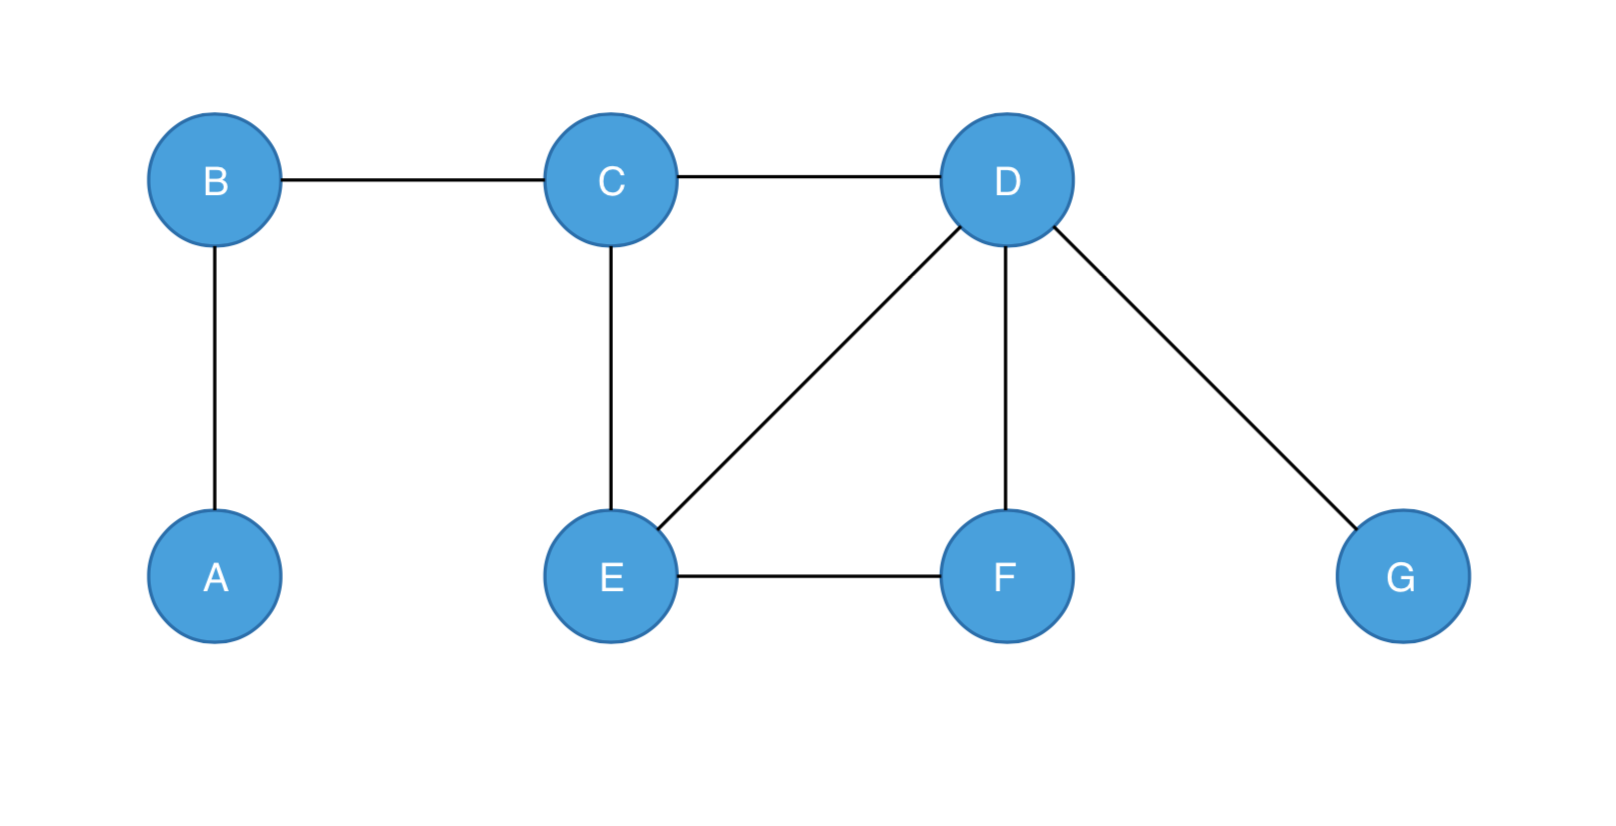
\includegraphics[height=4cm,width=9.5cm]{images/undirected.png}
	\caption{Undirected graph}
    \end{figure}
    \item \textbf{Directed graph}: When the set $E$ is represented as an ordered pair of vertices, it is called a directed graph or digraph. In a digraph, for some $x,y \in V(G)$, $(x,y) \neq (y,x)$.
    \begin{figure}[hbt!]
        \centering
	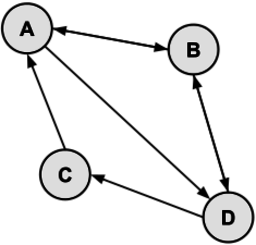
\includegraphics[height=4cm,width=7cm]{images/directed.png}
	\caption{Directed graph}
    \end{figure}
    \item \textbf{Multigraph}: If for any given vertices $x,y \in V(G)$, $\exists$ more than one edge $(x,y)$, then it is called a multigraph.
    \begin{figure}[hbt!]
        \centering
	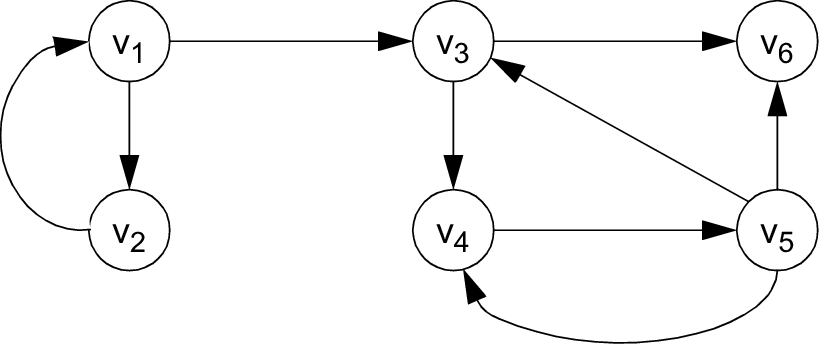
\includegraphics[height=4cm,width=9.5cm]{images/multi.png}
	\caption{Multigraph}
    \end{figure}
    \item \textbf{Pseudograph}: If for any given vertex, $x \in V(G)$, $\exists$ an edge $(x,x)$, that is, there is some edge $e$ that connects some vertex $x$ to itself.
    \begin{figure}[hbt!]
        \centering
	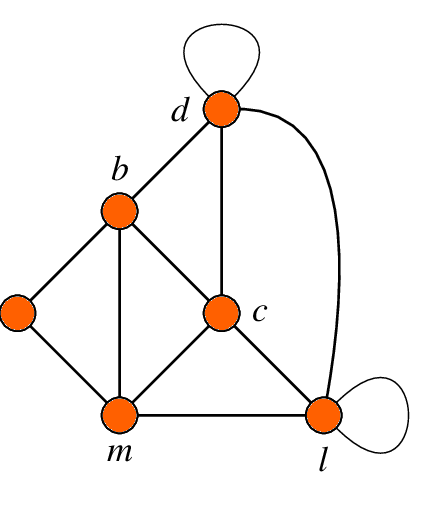
\includegraphics[height=3.82cm,width=7cm]{images/pseudo.png}
	\caption{Pseudograph}
    \end{figure}
    \item \textbf{Hypergraph}: If the edges of a graph are arbitrary subsets of vertices it is called hypergraph.
    \begin{figure}[hbt!]
        \centering
	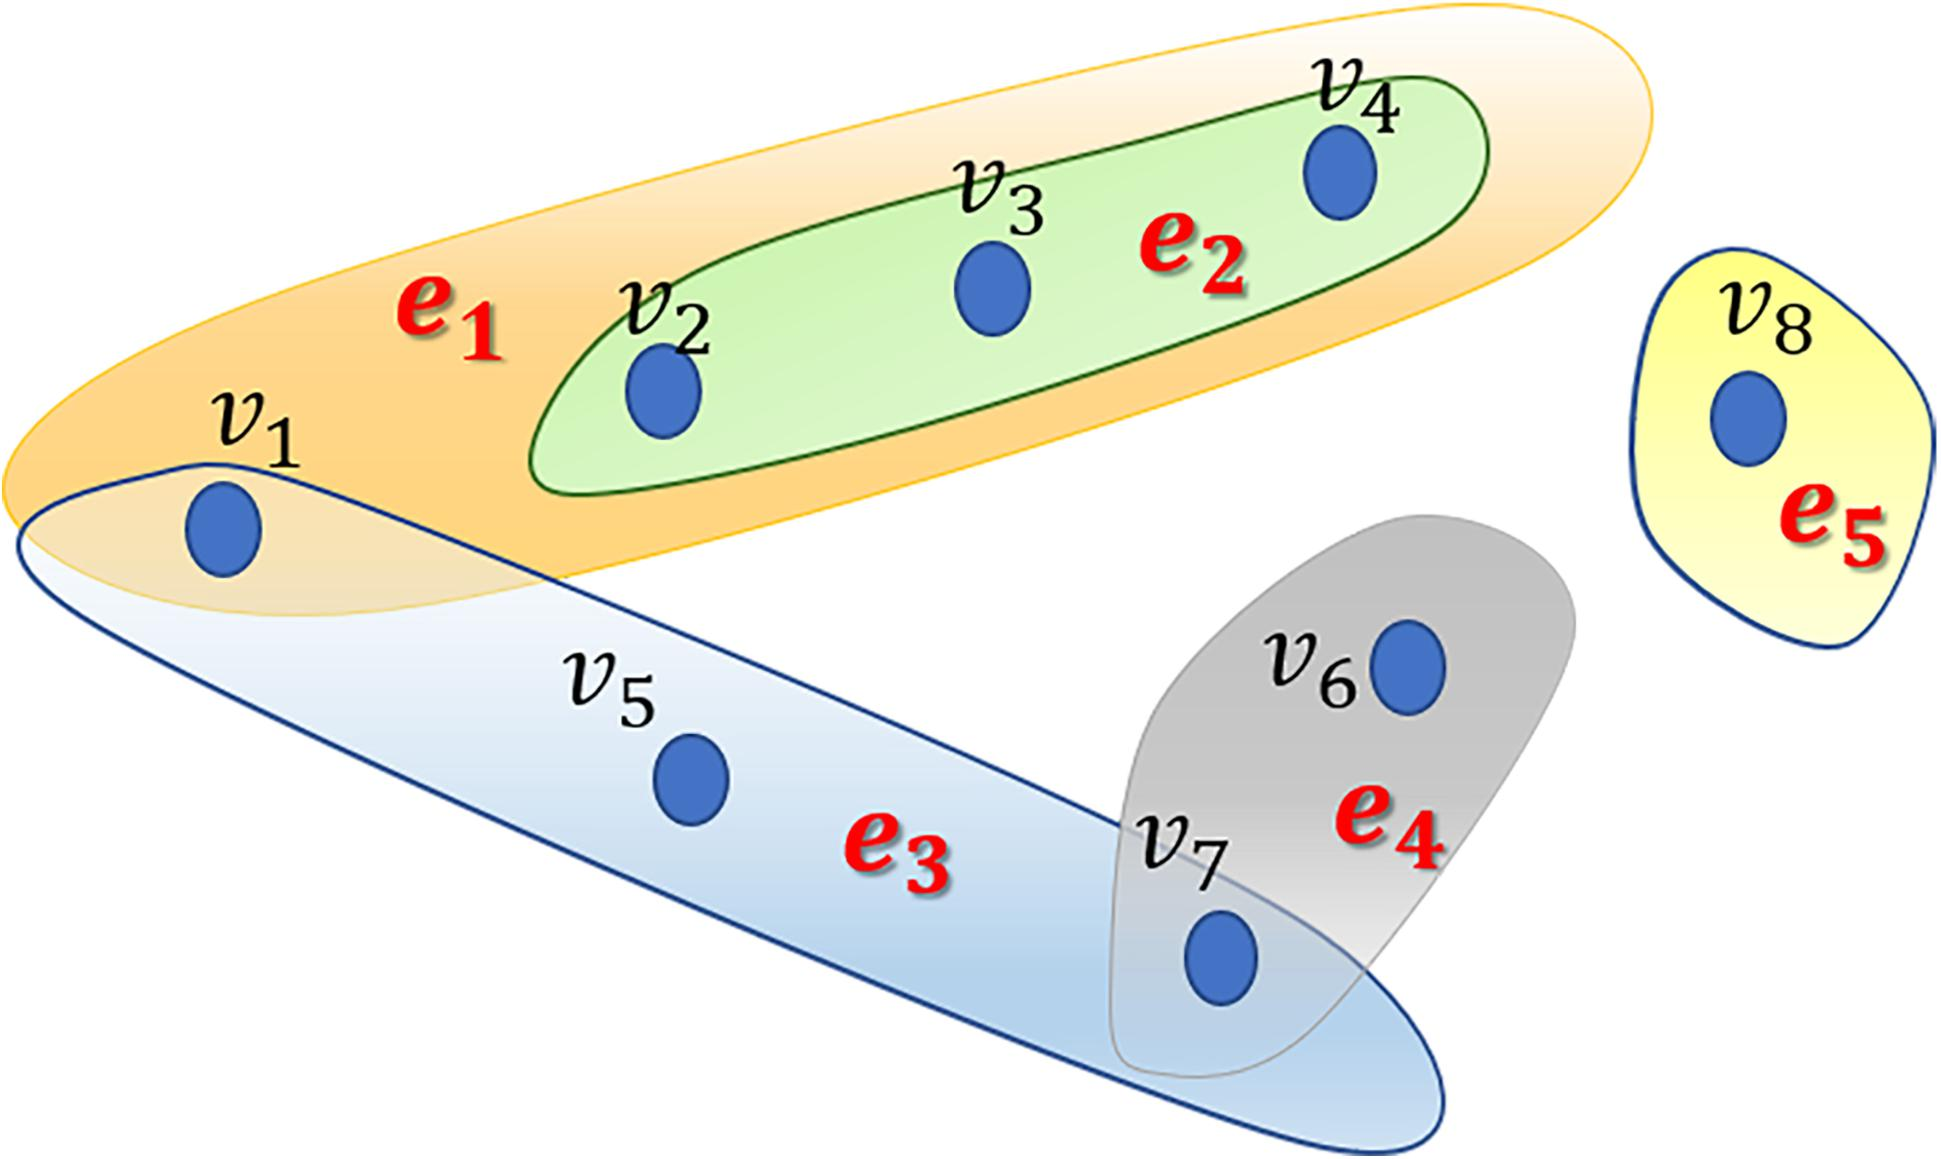
\includegraphics[height=4cm,width=9.5cm]{images/hyper.jpg}
	\caption{Hypergraph}
    \end{figure}
    \item \textbf{Infinite graph}: If the set $V$ or $E$ is infinite then it is called infinite graph.
\end{enumerate}
